\documentclass[10pt]{jarticle}
\usepackage{float}
\usepackage{adrobo_abst}
\usepackage[dvipdfmx]{graphicx}
\usepackage{amssymb,amsmath}
\usepackage{bm}
\usepackage[superscript]{cite}
\usepackage{enumerate}
\usepackage{url}
%\usepackage[absolute]{textpos}

\renewcommand\citeform[1]{(#1)}

\begin{document}
    
    \makeatletter
    \doctype{2023年度卒業論文概要}
    \title{人のような描き方ができる頭部の線画生成の研究}{}
    \etitle{The research for the drawing robot to generate line drawings of a person's head}{}
    
    \author{20C1119\hspace{.5zw}森田大雅}
    \eauthor{Hiromasa Morita}
    
    \makeatother
    
    \abstract{In the conventional study of the drawing robot, it is focused on the generated quality. However, we found the studies few, about the drawing order. In this study, we will consider how to draw like human.}
    
    \keywords{Mechanical Engineering, Image Proceesing, Forward Kinematics, Inverse Kinematics}
    
    \maketitle
    
    \supervisor{指導教員:藤江真也 教授}
    
    \section{緒\hspace{2zw}言}%===========================
	従来の描画ロボットの研究は生成された絵の結果について着目している研究が多い.
	本研究では, 人のような描き方をする描き順について検討する.

    \section{目的}
	描画ロボットの研究において, シンプルにエッジ抽出から人物画を描く手法\cite{1}や, エッジ抽出とハッチングから芸術的な人物画を鉛筆で描く手法\cite{2}, リモートユーザがタブレットを介してロボットに描かせる手法\cite{3}などが存在する.
	これらの研究では模写や芸術的な表現が可能になっているが, 人のような描き方を考慮した手法は見られない.
	そこで本研究では, ある画家が描いた頭部作品の画像から線画を生成し, その描き順ができるだけ人に近くなるようにペン先の軌道を求める手法を検討する.
    
    \section{システム構成}
	
	\subsection{ハードウェア}
	AdeeptのADA031を用いる. Arduinoで動作するため, 画像処理を行うのは難しい.
	そこで, 基盤をRaspberry\ Piに代え, ロボットアームのサーボモータに接続するためのブレッドボードやジャンパー線, 抵抗を用意した.
	
	\subsection{機構}
	本研究で用いるロボットは3軸のマニピュレータロボットである.
	servo1を原点, 各サーボモータの関節角を$\theta_1, \theta_2, \theta_3$, 各リンクの長さ$l_1, l_2, l_3, l_4$とし, 逆運動学問題を解く.
	また, リンク座標系を定める方法としてDH記法(Denavit-Hartenberg記法)を用いる.

    \begin{center}
        \begin{figure}[h]
            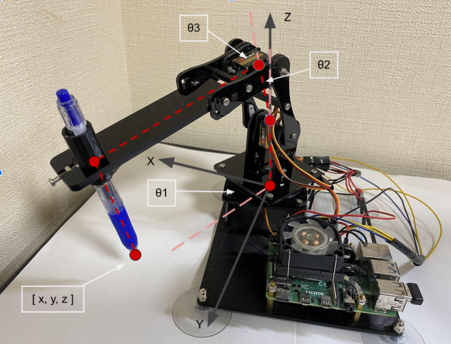
\includegraphics[width=0.40\textwidth]{img/002.png}
            \caption{各関節角と手先位置の関係}
            \label{manipulator}
        \end{figure}
    \end{center}
    
	\subsection{手先の位置と回転角の関係}
	順運動学, 逆運動学を用いてペン先の位置を各サーボモータの回転角を導出する.
	順運動学解より手先の位置が, また逆運動学解より各関節角がそれぞれ以下のように求まる.
	
	\scriptsize
	\begin{equation}
		\begin{array}{c}
			\begin{split}
				&  x  =  C_1(l_4C_{23}  +  l_3S_{23}  +  l_2S_2)\quad \\
				&  y  =  S_1(l_4C_{23}  +  l_3S_{23}  +  l_2S_2)\quad \\
				&  z  -  l_1  =  -l_4S_{23}  +  l_3C_{23}  +  l_2C_2\quad \\
			\end{split}
		\end{array}
	\end{equation}

	\begin{equation}
		\begin{array}{c}
			\begin{split}
				\theta_1  &  =\frac{1}{2}  cos^{-1}\biggl( \frac{x^2-y^2}{x^2+y^2} \biggr) \\
				\theta_2  &  = cos^{-1}\biggl( \frac{x^2+y^2+(z-l1)^2  +  l_2^2-l_3^2-l_4^2}{2l_2\sqrt{x^2+y^2+(z-l_1)^2}} \biggr)\\
				&\qquad\qquad  +  tan^{-1}\biggl( \frac{\sqrt{x^2+y^2}}{z-l1}\biggr) \\
				\theta_3  &  =cos^{-1}\biggl( \frac{x^2+y^2+(z-l1)^2 - l_4^2-l_3^2-l_2^2}{2l_2\sqrt{l_3^2+l_4^2}}\biggr)\\
				&\qquad\qquad + tan^{-1}\biggl( \frac{-l_4}{l_3}\biggr)\\
			\end{split}
		\end{array}
	\end{equation}
	
	\normalsize

	\subsection{エッジ抽出}
	画家ウィリアム・ブーグローの``金髪女の横顔''の画像を用いる.
	この画像は背景が白でシンプルである. そのため, 画像を読み込む際にノイズが少なく, 精確にエッジ抽出を行えると考えた.
	この画像から線画を生成するためにエッジを抽出する.
	線画の生成には, OpenCVのCannyのエッジ検出アルゴリズムを用いる.	
	
	\subsection{経路の求め方}
	領域と端点を用いて線の経路を求める.
	頭部の線画を描くパターンを調べた.
	著者は顔の輪郭から始まり, 首や目, 鼻などの細部に移って描いていく.
	全体から描くことによりパーツの位置を決めやすいからだと考えられる.
	また, 右利きの場合, 開始点は左側が多かった.
	ペンを右側に傾けて持つため, 時計周りに円を描くのが描きやすいからだと考えられる.
	半時計周りの場合, 6時から12時までの区間を描くには手を少し持ち上げて描く必要がある.
    そのため, 寝かせたまま描くことのできる時計周りより不安定になる.
	
	\subsection{スタート地点の決め方}
	左側から描くためにある大きさの領域を用意した.
	領域は正方形で, 左上の位置が横全体の$\frac{1}{8}$, 縦全体の$\frac{1}{3}$に, サイズが横全体の$\frac{1}{4}$になるように設定した.
	領域が頭部の左側にあるか2つの画像で確かめた.
	\\\ この領域を縦方向にスキャンし, 最初にエッジの画素にぶつかった位置をスタート地点とする.

    \begin{center}
        \begin{figure}[h]
            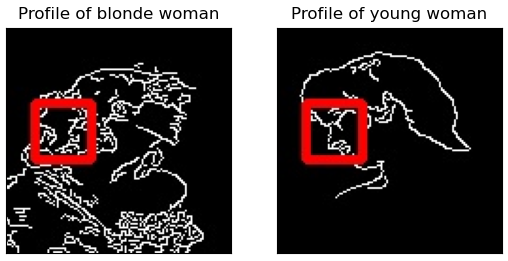
\includegraphics[width=0.40\textwidth]{img/003.png}
            \caption{領域の位置の確認}
            \label{the position of a region}
        \end{figure}
    \end{center}
	

	\subsection{端点の検出と線の追跡法}
	Fig.1ではエッジは全て繋がって見えるが, 実際には途切れている. そのため, これをそのままロボットに与えると点線になる.
	そこで端点を用いる.
	線の画素を辿り, 端点まで来たら次に近くの端点に移動して描いていく.
	この処理を行うことで, 点線を描いていくことになるが, 近似的に線を描く動作が実現できる.
  \\\  
	線の辿り方は, ある線の画素から隣に線の画素があるかを探し, 線の画素があれば移動し, なければ最も近く通過していない端点へと移動する.
	これを線の画素がなくなるまで繰り返す.
	
	\section{実験}
	経路を求める方法として, ラスタスキャンと端点を用いた方法のどちらが人のような描き方に近いかを比較するため, 10枚の画像を使って8人にアンケートを取った.

	\subsection{結果}
	下の表はアンケート結果である. ほとんどの場合でラスタスキャンの方が人に近いという結果が出た. 

\begin{table}[h]
  \caption{アンケート結果\label{アンケート結果}}
  \label{tab:sample-tab}
  \begin{center}
      \vskip 1zh
      \small
      \begin{tabular}{c|c|c} \hline
                         & ラスタスキャン(\%)   & 端点(\%)  \\ \hline
        画像1            & 62.5   				& 37.5   \\ \hline
        画像2            & 62.5	  				& 37.5   \\ \hline
        画像3            & 75.0   				& 25.0   \\ \hline
        画像4            & 75.0   				& 25.0   \\ \hline
        画像5            & 50.0   				& 50.0   \\ \hline
        画像6            & 62.5   				& 37.5   \\ \hline
        画像7            & 62.5   				& 37.5   \\ \hline
        画像8            & 25.0   				& 75.0   \\ \hline
        画像9            & 75.0   				& 25.0   \\ \hline
        画像10           & 75.0   				& 25.0   \\ \hline
      \end{tabular}
  \end{center}
\end{table}  

	\subsection{考察}
	最も近い端点に移動すれば, 近似的に線を描けると仮定したが, 交点を考慮する必要があった. そのため, 本来とは違う軌道になることが多くなったと考えられる.
	また, エッジとノイズはトレードオフ関係にある[\cite{4}]ため, エッジを用いて線画を描くなら, 途切れた線を補間する必要があると考えられる. 
	
	\section{結\hspace{2zw}言}%===========================
	本手法では, 端点を用いて人のような描き方ができるのかを調査した.
	比較結果はラスタスキャンの方が投票数が多く, 望ましい結果が得られなかった. 
	交点の考慮や途切れた線の補間が必要だった. 
	
    \vspace{5truemm}
    {\footnotesize
        \begin{thebibliography}{99}
            
            \bibitem{1}
            M. Pichkalev, R. Lavrenov, R. Safin and K. -H. Hsia, "Face Drawing by KUKA 6 Axis Robot Manipulator," 2019 12th International Conference on Developments in eSystems Engineering (DeSE), Kazan, Russia, 2019, pp. 709-714, doi: 10.1109/DeSE.2019.00132.

			\bibitem{2}
            Felix Fisgus, Joris Wegner: ``Pankraz Piktograph'', 
            \url{https://felixfisgus.de/work/017\_pankraz\_piktograph}
            (参照日 2023年7月29日) .
            
			\bibitem{3}
            Shubham Agarwal, Sarvesh S. S. Rawat, V Sumathi: ``A drawing robotic hand based on inverse kinematics'', 
            International Conference on Information Communication and Embedded Systems (ICICES2014), Chennai, India, 2014, pp. 1-5, doi: 10.1109/ICICES.2014.7034005.
           \bibitem{4}
		   D. Dhillon and R. Chouhan, "Enhanced Edge Detection Using SR-Guided Threshold Maneuvering and Window Mapping: Handling Broken Edges and Noisy Structures in Canny Edges," in IEEE Access, vol. 10, pp. 11191-11205, 2022, doi: 10.1109/ACCESS.2022.3145428.
            
        \end{thebibliography}
    }
    \normalsize
    
\end{document}

